% Options for packages loaded elsewhere
% Options for packages loaded elsewhere
\PassOptionsToPackage{unicode}{hyperref}
\PassOptionsToPackage{hyphens}{url}
%
\documentclass[
  ignorenonframetext,
  aspectratio=169,
  handout]{beamer}
\newif\ifbibliography
\usepackage{pgfpages}
\setbeamertemplate{caption}[numbered]
\setbeamertemplate{caption label separator}{: }
\setbeamercolor{caption name}{fg=normal text.fg}
\beamertemplatenavigationsymbolsempty
% remove section numbering
\setbeamertemplate{part page}{
  \centering
  \begin{beamercolorbox}[sep=16pt,center]{part title}
    \usebeamerfont{part title}\insertpart\par
  \end{beamercolorbox}
}
\setbeamertemplate{section page}{
  \centering
  \begin{beamercolorbox}[sep=12pt,center]{section title}
    \usebeamerfont{section title}\insertsection\par
  \end{beamercolorbox}
}
\setbeamertemplate{subsection page}{
  \centering
  \begin{beamercolorbox}[sep=8pt,center]{subsection title}
    \usebeamerfont{subsection title}\insertsubsection\par
  \end{beamercolorbox}
}
% Prevent slide breaks in the middle of a paragraph
\widowpenalties 1 10000
\raggedbottom
\AtBeginPart{
  \frame{\partpage}
}
\AtBeginSection{
  \ifbibliography
  \else
    \frame{\sectionpage}
  \fi
}
\AtBeginSubsection{
  \frame{\subsectionpage}
}
\usepackage{iftex}
\ifPDFTeX
  \usepackage[T1]{fontenc}
  \usepackage[utf8]{inputenc}
  \usepackage{textcomp} % provide euro and other symbols
\else % if luatex or xetex
  \usepackage{unicode-math} % this also loads fontspec
  \defaultfontfeatures{Scale=MatchLowercase}
  \defaultfontfeatures[\rmfamily]{Ligatures=TeX,Scale=1}
\fi
\usepackage{lmodern}

\ifPDFTeX\else
  % xetex/luatex font selection
\fi
% Use upquote if available, for straight quotes in verbatim environments
\IfFileExists{upquote.sty}{\usepackage{upquote}}{}
\IfFileExists{microtype.sty}{% use microtype if available
  \usepackage[]{microtype}
  \UseMicrotypeSet[protrusion]{basicmath} % disable protrusion for tt fonts
}{}
\makeatletter
\@ifundefined{KOMAClassName}{% if non-KOMA class
  \IfFileExists{parskip.sty}{%
    \usepackage{parskip}
  }{% else
    \setlength{\parindent}{0pt}
    \setlength{\parskip}{6pt plus 2pt minus 1pt}}
}{% if KOMA class
  \KOMAoptions{parskip=half}}
\makeatother


\usepackage{longtable,booktabs,array}
\newcounter{none} % for unnumbered tables
\usepackage{calc} % for calculating minipage widths
\usepackage{caption}
% Make caption package work with longtable
\makeatletter
\def\fnum@table{\tablename~\thetable}
\makeatother
\usepackage{graphicx}
\makeatletter
\newsavebox\pandoc@box
\newcommand*\pandocbounded[1]{% scales image to fit in text height/width
  \sbox\pandoc@box{#1}%
  \Gscale@div\@tempa{\textheight}{\dimexpr\ht\pandoc@box+\dp\pandoc@box\relax}%
  \Gscale@div\@tempb{\linewidth}{\wd\pandoc@box}%
  \ifdim\@tempb\p@<\@tempa\p@\let\@tempa\@tempb\fi% select the smaller of both
  \ifdim\@tempa\p@<\p@\scalebox{\@tempa}{\usebox\pandoc@box}%
  \else\usebox{\pandoc@box}%
  \fi%
}
% Set default figure placement to htbp
\def\fps@figure{htbp}
\makeatother





\setlength{\emergencystretch}{3em} % prevent overfull lines

\providecommand{\tightlist}{%
  \setlength{\itemsep}{0pt}\setlength{\parskip}{0pt}}



 


\makeatletter
\@ifpackageloaded{caption}{}{\usepackage{caption}}
\AtBeginDocument{%
\ifdefined\contentsname
  \renewcommand*\contentsname{Table of contents}
\else
  \newcommand\contentsname{Table of contents}
\fi
\ifdefined\listfigurename
  \renewcommand*\listfigurename{List of Figures}
\else
  \newcommand\listfigurename{List of Figures}
\fi
\ifdefined\listtablename
  \renewcommand*\listtablename{List of Tables}
\else
  \newcommand\listtablename{List of Tables}
\fi
\ifdefined\figurename
  \renewcommand*\figurename{Figure}
\else
  \newcommand\figurename{Figure}
\fi
\ifdefined\tablename
  \renewcommand*\tablename{Table}
\else
  \newcommand\tablename{Table}
\fi
}
\@ifpackageloaded{float}{}{\usepackage{float}}
\floatstyle{ruled}
\@ifundefined{c@chapter}{\newfloat{codelisting}{h}{lop}}{\newfloat{codelisting}{h}{lop}[chapter]}
\floatname{codelisting}{Listing}
\newcommand*\listoflistings{\listof{codelisting}{List of Listings}}
\makeatother
\makeatletter
\makeatother
\makeatletter
\@ifpackageloaded{caption}{}{\usepackage{caption}}
\@ifpackageloaded{subcaption}{}{\usepackage{subcaption}}
\makeatother

\usepackage{bookmark}
\IfFileExists{xurl.sty}{\usepackage{xurl}}{} % add URL line breaks if available
\urlstyle{same}
\hypersetup{
  pdftitle={Atomic Orbitals},
  pdfauthor={Davit Potoyan},
  hidelinks,
  pdfcreator={LaTeX via pandoc}}


\title{\texorpdfstring{Atomic Orbitals}{Atomic Orbitals}}
\subtitle{\texorpdfstring{Chem 3240 · Lecture
5.2}{Chem 3240 · Lecture 5.2}}
\author{Davit Potoyan}
\date{}

\begin{document}
\frame{\titlepage}


\begin{frame}
\begin{block}{What Is an Orbital?}
\protect\phantomsection\label{what-is-an-orbital}
\begin{itemize}
\tightlist
\item
  A \textbf{one-electron wavefunction} is called an \textbf{orbital}.
\item
  For the hydrogen atom it is an \textbf{atomic orbital (AO)}, exact for
  H-like atoms.
\end{itemize}

\[\psi_{n\ell m_\ell}(r,\theta,\phi) = R_{n\ell}(r)\,Y_{\ell m_\ell}(\theta,\phi)\]

\begin{itemize}
\tightlist
\item
  Splits cleanly into a \textbf{radial} part and an \textbf{angular}
  part.
\end{itemize}
\end{block}

\begin{block}{Three Quantum Numbers}
\protect\phantomsection\label{three-quantum-numbers}
\begin{itemize}
\tightlist
\item
  \textbf{Principal:} \(n = 1, 2, 3, \ldots\)
\end{itemize}

\begin{itemize}
\tightlist
\item
  \textbf{Orbital angular momentum:} \(\ell = 0, 1, 2, \ldots, n-1\)
\end{itemize}

\begin{itemize}
\tightlist
\item
  \textbf{Magnetic:} \(m_\ell = -\ell, -\ell+1, \ldots, \ell\)
\end{itemize}

\begin{itemize}
\tightlist
\item
  Each valid triple labels \textbf{one} orbital.
\end{itemize}
\end{block}

\begin{block}{Where Is the Electron?}
\protect\phantomsection\label{where-is-the-electron}
\begin{itemize}
\tightlist
\item
  Probability over the full 3D volume:
\end{itemize}

\[|\psi|^2 dV = \big|R_{n\ell}(r)\big|^2 \cdot \big|Y_{\ell m_\ell}(\theta,\phi)\big|^2 \cdot r^2\sin\theta \, dr \, d\theta \, d\phi\]

\begin{itemize}
\tightlist
\item
  The \(r^2\) factor reshapes the radial picture.
\end{itemize}
\end{block}

\begin{block}{Radial Probability}
\protect\phantomsection\label{radial-probability}
\begin{columns}[T]
\begin{column}{0.5\linewidth}
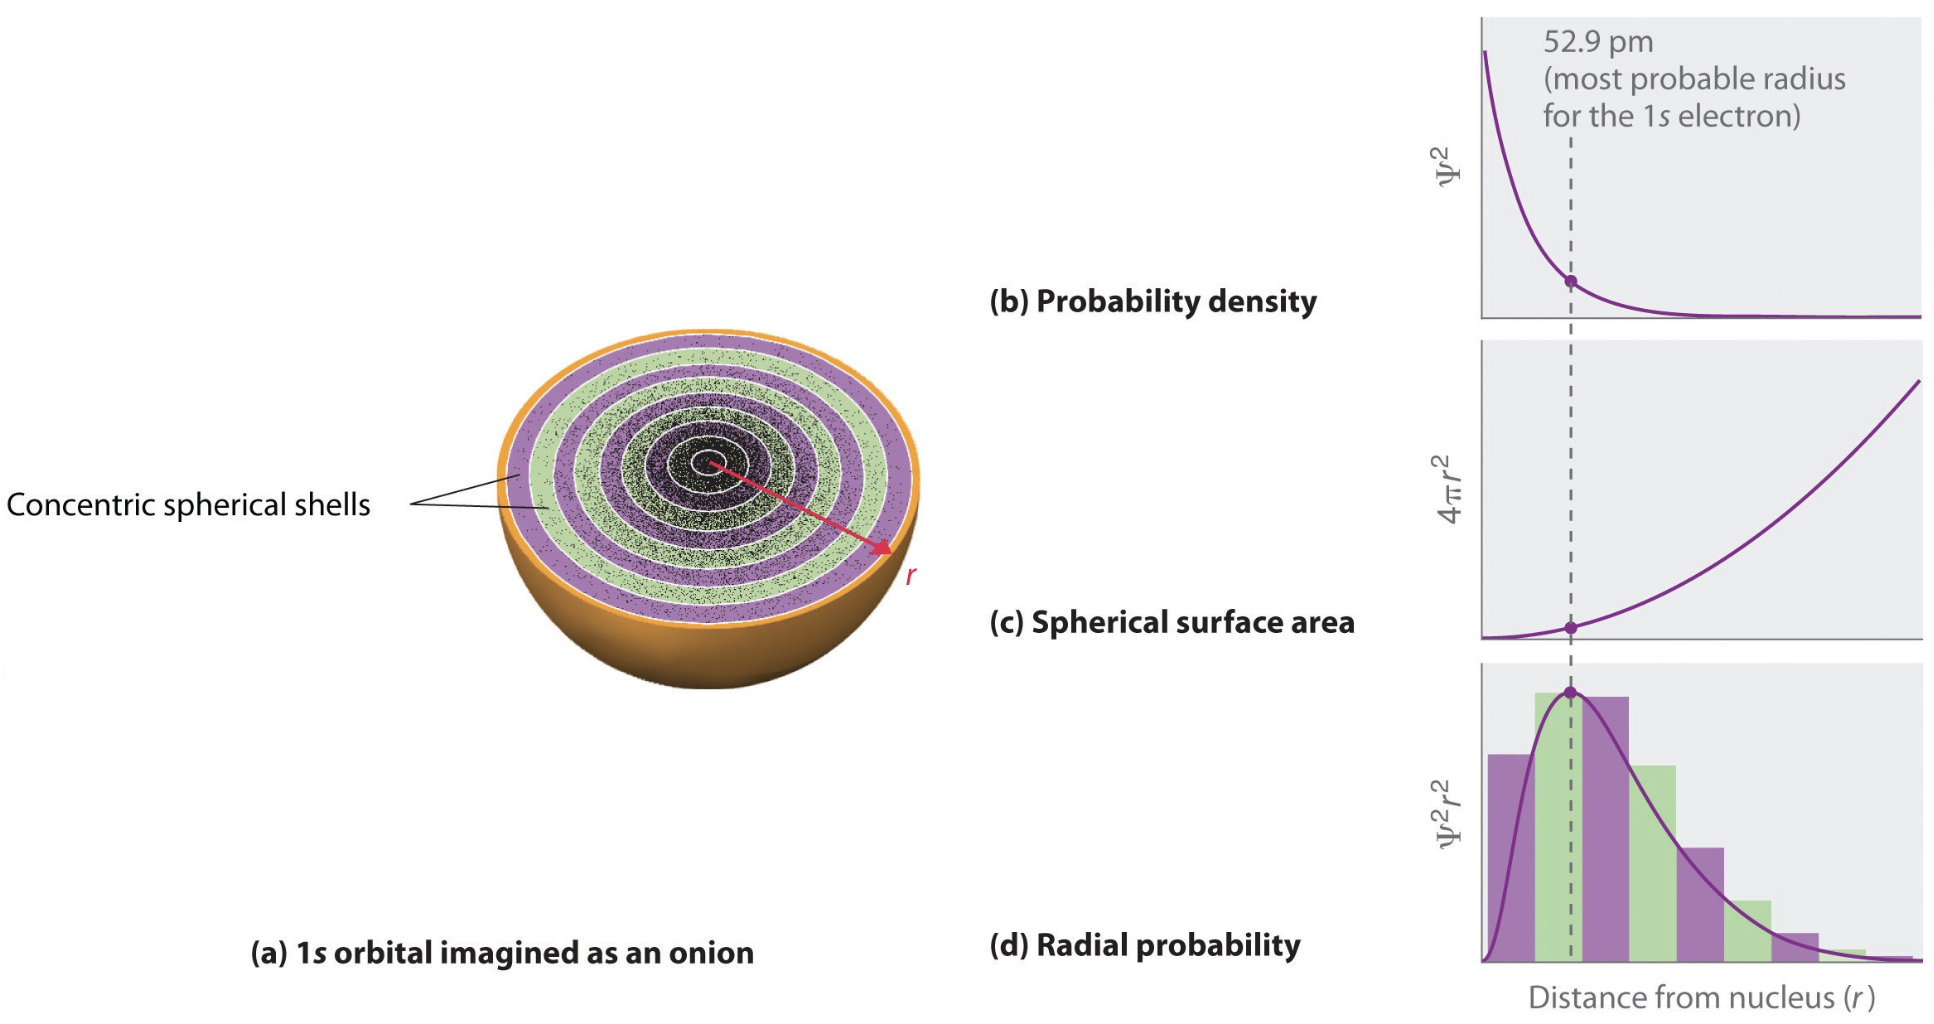
\includegraphics[width=1\linewidth,height=\textheight,keepaspectratio]{../../ch05/images/AO_0.png}
\end{column}

\begin{column}{0.5\linewidth}
\[P_r(r) = r^2\big|R_{n\ell}(r)\big|^2\]

\begin{itemize}
\tightlist
\item
  Peaks mark the \textbf{most probable distance} from the nucleus.
\end{itemize}

\begin{itemize}
\tightlist
\item
  For the \(1s\) orbital the peak sits at the \textbf{Bohr radius}
  \(a_0\).
\end{itemize}
\end{column}
\end{columns}
\end{block}

\begin{block}{How Far Out?}
\protect\phantomsection\label{how-far-out}
\begin{itemize}
\tightlist
\item
  Average distance grows with \(n\):
\end{itemize}

\[\langle r\rangle_{nl} = \frac{n^2 a_0}{Z}\left\{ 1 + \frac{1}{2}\left[ 1 - \frac{l(l+1)}{n^2}\right]\right\}\]

\begin{itemize}
\tightlist
\item
  Larger \(n\): electron \textbf{moves outward}.
\item
  Larger \(Z\): electron \textbf{pulled inward}.
\end{itemize}

\begin{itemize}
\tightlist
\item
  Expectation value \(\langle r\rangle\) is \textbf{not} the most
  probable \(r\).
\end{itemize}
\end{block}

\begin{block}{Counting Nodes}
\protect\phantomsection\label{counting-nodes}
\begin{itemize}
\tightlist
\item
  \textbf{Radial} nodes: \(n - \ell - 1\)
\end{itemize}

\begin{itemize}
\tightlist
\item
  \textbf{Angular} nodes: \(\ell\)
\end{itemize}

\begin{itemize}
\tightlist
\item
  \textbf{Total} nodes: \(n - 1\)
\end{itemize}

\begin{itemize}
\tightlist
\item
  More nodes mean more \textbf{curvature} and higher energy.
\end{itemize}
\end{block}

\begin{block}{Angular Shapes}
\protect\phantomsection\label{angular-shapes}
\begin{columns}[T]
\begin{column}{0.5\linewidth}
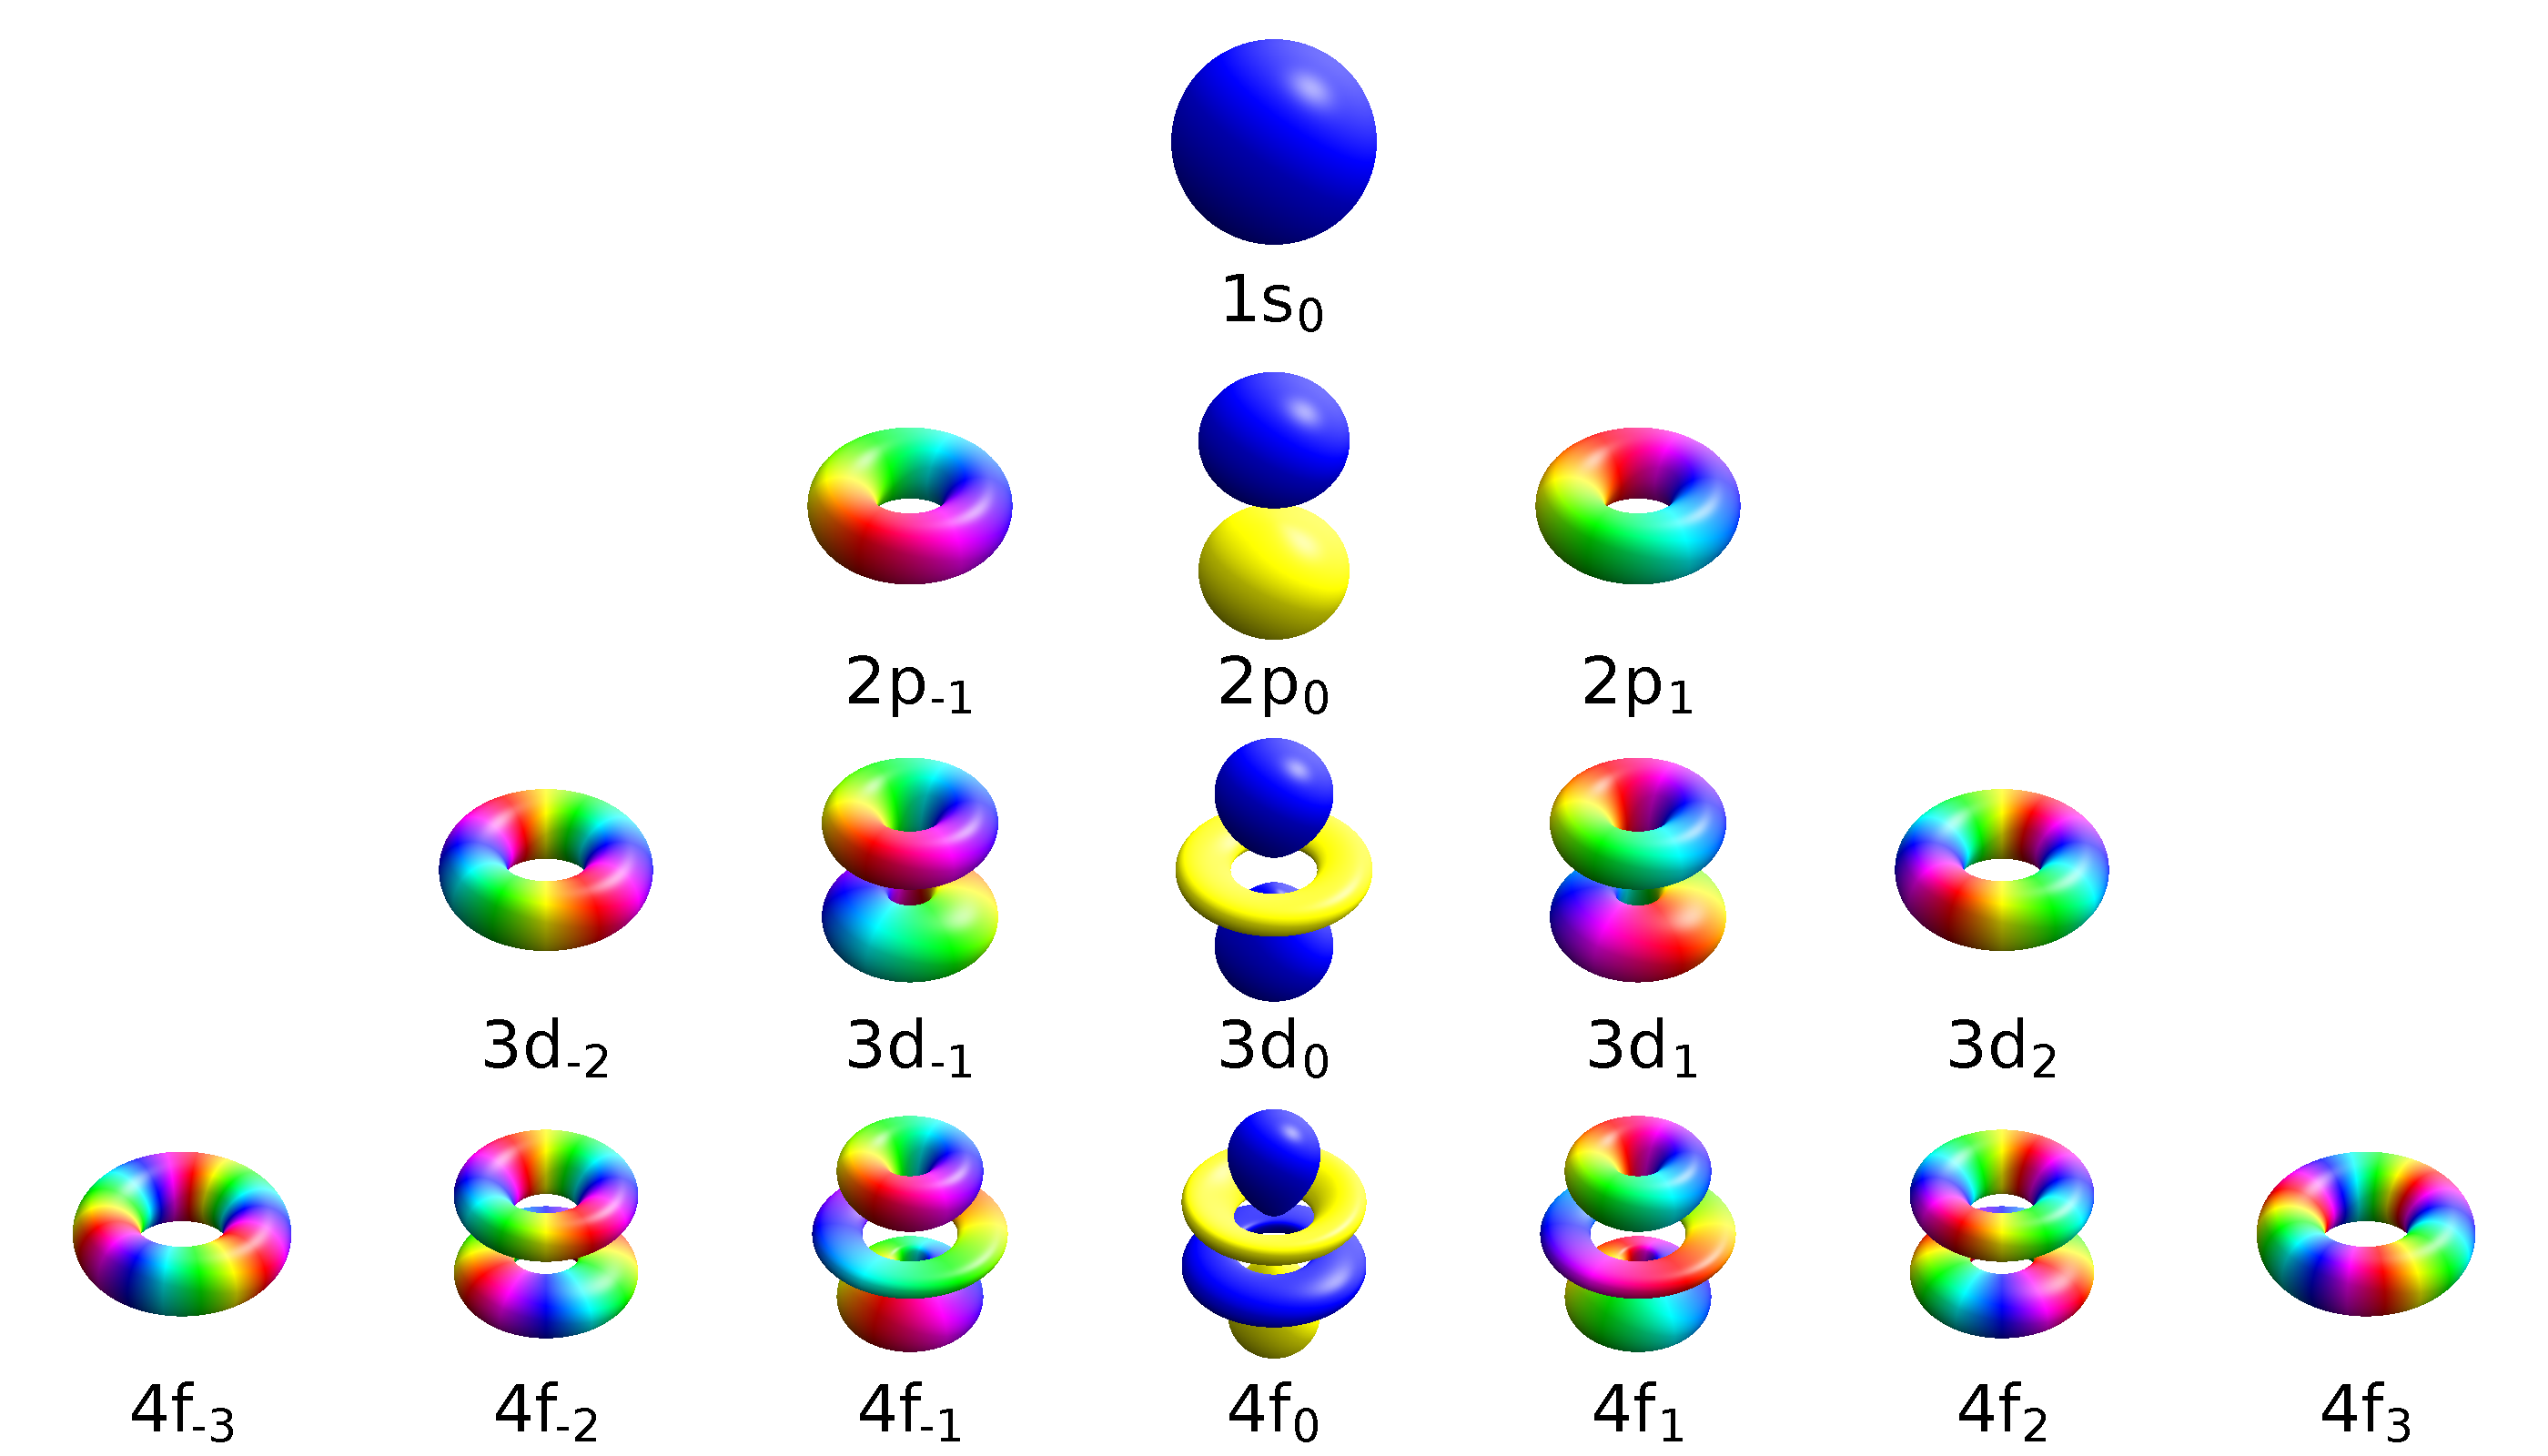
\includegraphics[width=1\linewidth,height=\textheight,keepaspectratio]{../../ch05/images/AO.png}
\end{column}

\begin{column}{0.5\linewidth}
\[P_\Omega(\theta,\phi) = \big|Y_{\ell m_\ell}(\theta,\phi)\big|^2\]

\begin{itemize}
\tightlist
\item
  \(s\) orbitals (\(\ell = 0\)) are \textbf{isotropic}:
  \(P_\Omega = \tfrac{1}{4\pi}\).
\end{itemize}

\begin{itemize}
\tightlist
\item
  \(p, d, \ldots\) have \textbf{angular nodes} that carve the lobes.
\end{itemize}
\end{column}
\end{columns}
\end{block}

\begin{block}{Real vs Complex Orbitals}
\protect\phantomsection\label{real-vs-complex-orbitals}
\begin{columns}[T]
\begin{column}{0.5\linewidth}
\includegraphics[width=1\linewidth,height=\textheight,keepaspectratio]{../../ch05/images/Orbital_p1-px_animation.gif}
\end{column}

\begin{column}{0.5\linewidth}
\begin{itemize}
\tightlist
\item
  Degenerate \(\ell > 0\) states allow \textbf{free recombination}.
\end{itemize}

\[p_x \propto \sin\theta\cos\phi \propto x\]
\[p_y \propto \sin\theta\sin\phi \propto y\] \[p_z = p_0\]

\begin{itemize}
\tightlist
\item
  Same density, \textbf{different frame}.
\end{itemize}
\end{column}
\end{columns}
\end{block}

\begin{block}{Pointing the Lobes}
\protect\phantomsection\label{pointing-the-lobes}
\begin{itemize}
\tightlist
\item
  Combining \(p_x, p_y, p_z\) aims a lobe in \textbf{any direction}.
\item
  Five degenerate \(d\) orbitals follow the same recipe:
\end{itemize}

\[d_{x^2 - y^2} = \tfrac{1}{\sqrt{2}}\left(d_{+2} + d_{-2}\right), \quad d_{xy} = -\tfrac{i}{\sqrt{2}}\left( d_{+2} - d_{-2}\right)\]
\[d_{xz} = -\tfrac{1}{\sqrt{2}}\left( d_{+1} - d_{-1}\right), \quad d_{yz} = \tfrac{i}{\sqrt{2}}\left( d_{+1} + d_{-1}\right)\]
\[d_{z^2} = d_0\]
\end{block}

\begin{block}{Putting It Together}
\protect\phantomsection\label{putting-it-together}
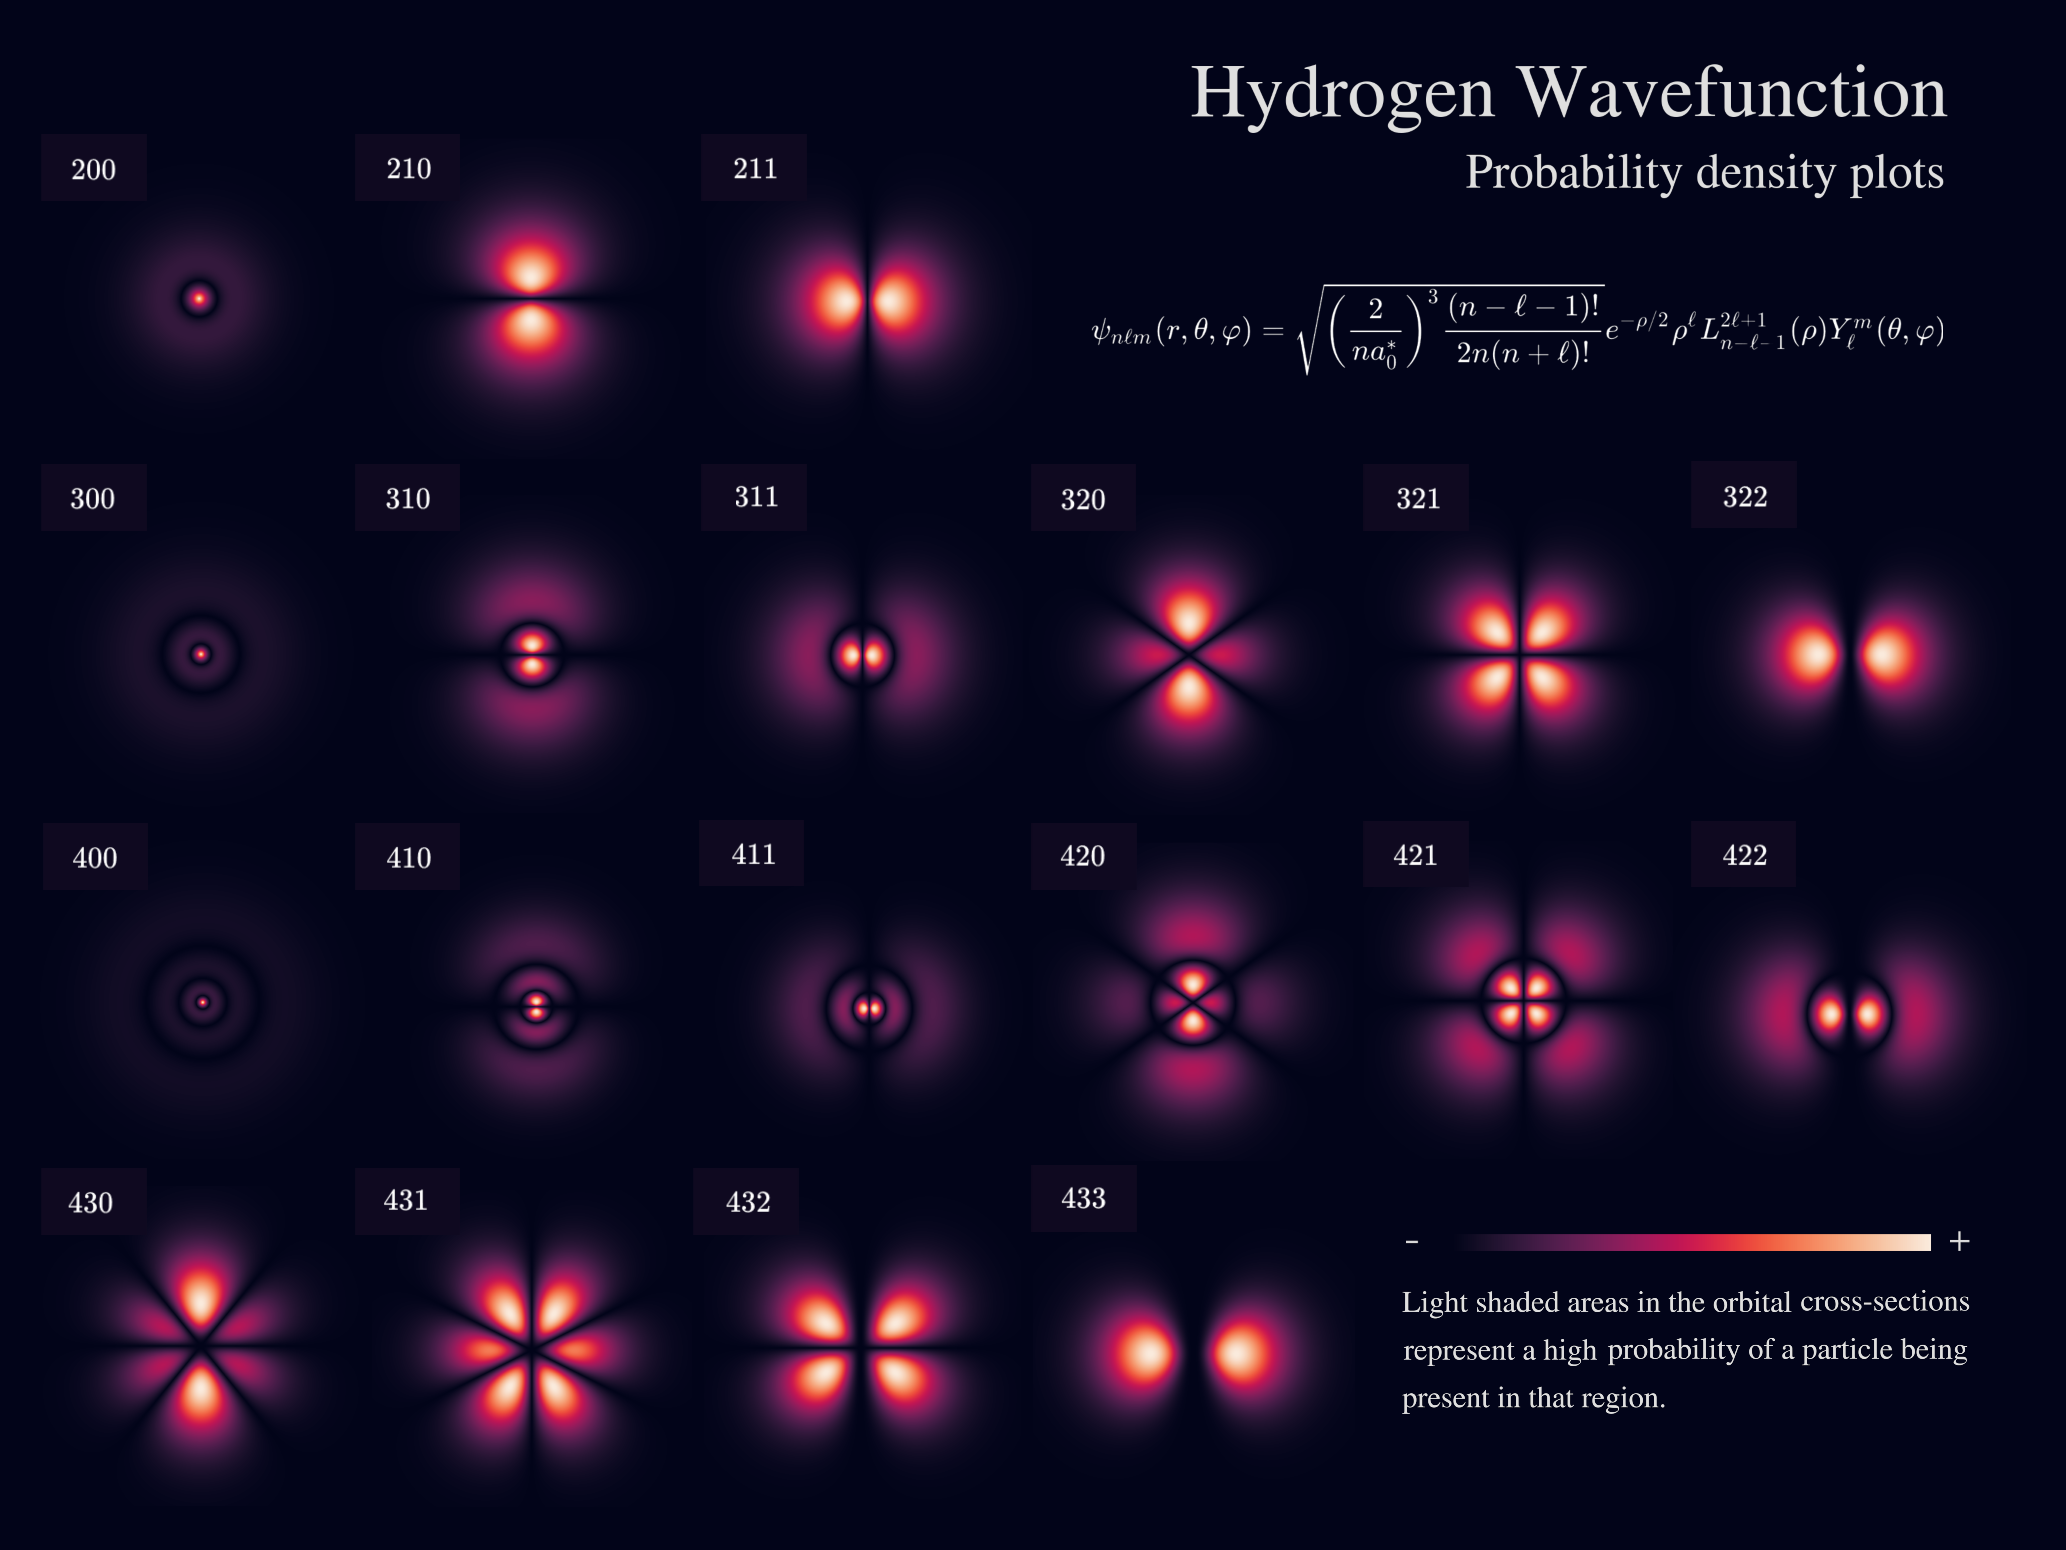
\includegraphics[width=0.78\linewidth,height=\textheight,keepaspectratio]{../../ch05/images/hydrogen_probability_densities.png}

\begin{itemize}
\tightlist
\item
  Cross sections of \(|\psi_{n\ell m}|^2\): \textbf{radial reach} times
  \textbf{angular shape}.
\end{itemize}
\end{block}
\end{frame}

\begin{frame}{Takeaway}
\protect\phantomsection\label{takeaway}
\begin{quote}
An atomic orbital factors as
\(\psi = R_{n\ell}(r)\,Y_{\ell m_\ell}(\theta,\phi)\), labeled by \(n\),
\(\ell\), \(m_\ell\). The radial part sets \textbf{how far}
(\(n - \ell - 1\) nodes) and the angular part sets the \textbf{shape}
(\(\ell\) nodes), for \(n - 1\) nodes in all.
\end{quote}
\end{frame}




\end{document}
